\subsection{Living rooms}
\label{sec:application:building_the_model:living_rooms}

In the final step, a last data field is introduced. In this step, the $.\type{House}$ class is enriched with an $\type{living\_room}$ field and its values. As before, \cref{subsec:library_of_transformations:type_level_transformations:data_fields} is used to introduce the field, while on the instance level, \cref{subsec:library_of_transformations:instance_level_transformations:data_field_values} is used to introduce the values.

The $classtype$ of the new field is $.\type{House}$, as the field will be defined for houses. The $name$ of the new field is $\type{living\_room}$ and the $fieldtype$ is $\type{bool}$. The set of objects of which the value is set is is equal to all house objects, so $objects = \{TR, BHP\}$. The function for $obids$ returns the existing identifier of each of these objects. The $values$ function is defined as follows:
\begin{align*}
    values = \{&(TR, \text{false}), (BHP, \text{true})\}
\end{align*}

The following model is obtained:

\LTXtable{\textwidth}{tex/06_application/02_building_the_model/tables/15_living_rooms.tex}

\begin{figure}[p]
    \centering
    \begin{subfigure}{0.98\textwidth}
        \centering
        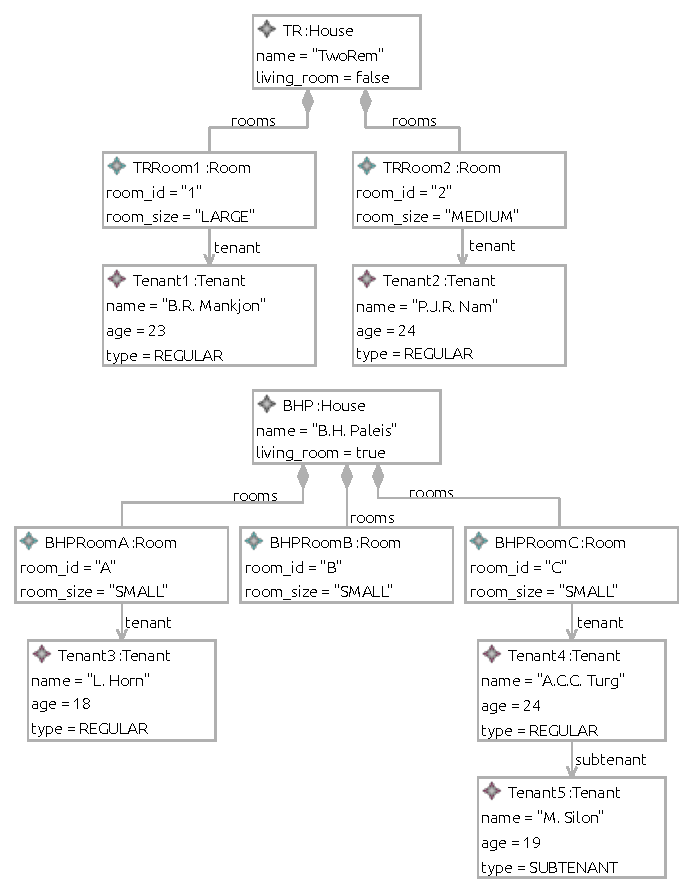
\includegraphics{images/06_application/instance_model/step15.pdf}
        \caption{Instance Model $Im_{15}$}
        \label{fig:application:building_the_model:living_rooms:ecore:instance_model}
    \end{subfigure}
    \\
    \begin{subfigure}{0.98\textwidth}
        \centering
        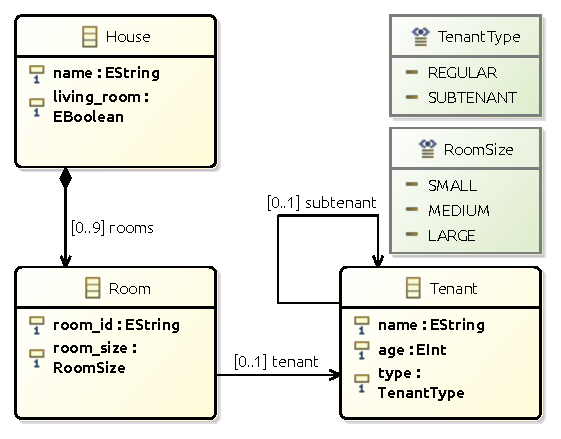
\includegraphics{images/06_application/type_model/step15.pdf}
        \caption{Type Model $Tm_{15}$}
        \label{fig:application:building_the_model:living_rooms:ecore:type_model}
    \end{subfigure}
    \caption{The Ecore model after the final step}
    \label{fig:application:building_the_model:living_rooms:ecore}
\end{figure}

\begin{figure}[p]
    \centering
    \begin{subfigure}{0.98\textwidth}
        \centering
        % To use this figure in your LaTeX document
% import the package groove/resources/groove2tikz.sty
%
\begin{tikzpicture}[scale=\tikzscale,name prefix=step15-]
\node[type_node] (n0) at (0.740, -0.400) {\ml{\textbf{House}\\living\_room: \textbf{bool}\\name: \textbf{string}}};
\node[type_node] (n1) at (0.730, -1.585) {\ml{\textbf{Room}\\room\_id: \textbf{string}}};
\node[type_node] (n2) at (2.380, -0.560) {\ml{\textbf{RoomSize}\\\textit{LARGE}\\\textit{MEDIUM}\\\textit{SMALL}}};
\node[type_node] (n3) at (2.500, -1.590) {\ml{\textbf{Tenant}\\age: \textbf{int}\\name: \textbf{string}}};
\node[abstract_node] (n4) at (4.710, -0.980) {\ml{\textit{\textbf{TenantType}}}};
\node[type_node] (n5) at (3.810, -0.320) {\ml{\textbf{TenantType\$REGULAR}}};
\node[type_node] (n6) at (5.680, -0.320) {\ml{\textbf{TenantType\$SUBTENANT}}};

\path[basic_edge, composite](n0.south -| 0.730, -1.585) -- node[lab] {\ml{rooms}} (n1) ;
\path[basic_edge] (n1)  -- node[lab] {\ml{room\_size}} (n2) ;
\path[basic_edge] (n3)  -- node[lab] {\ml{type}} (n4) ;
\path[basic_edge](n1.east |- 2.500, -1.590) -- node[lab] {\ml{tenant}} (n3) ;
\path[basic_edge] (n3)  -- (3.430, -2.140) --  (n3) 
node[lab] at (3.430, -2.140) {\ml{subtenant}};
\path[subtype_edge] (n6)  --  (n4) ;
\path[subtype_edge] (n5)  --  (n4) ;
\end{tikzpicture}

        \caption{Instance Graph $IG_{15}$}
        \label{fig:application:building_the_model:living_rooms:groove:instance_graph}
    \end{subfigure}
    \\
    \begin{subfigure}{0.98\textwidth}
        \centering
        % To use this figure in your LaTeX document
% import the package groove/resources/groove2tikz.sty
%
\begin{tikzpicture}[scale=\tikzscale,name prefix=step15-]
\node[type_node] (n0) at (0.740, -0.400) {\ml{\textbf{House}\\living\_room: \textbf{bool}\\name: \textbf{string}}};
\node[type_node] (n1) at (0.730, -1.585) {\ml{\textbf{Room}\\room\_id: \textbf{string}}};
\node[type_node] (n2) at (2.380, -0.560) {\ml{\textbf{RoomSize}\\\textit{LARGE}\\\textit{MEDIUM}\\\textit{SMALL}}};
\node[type_node] (n3) at (2.500, -1.590) {\ml{\textbf{Tenant}\\age: \textbf{int}\\name: \textbf{string}}};
\node[abstract_node] (n4) at (4.710, -0.980) {\ml{\textit{\textbf{TenantType}}}};
\node[type_node] (n5) at (3.810, -0.320) {\ml{\textbf{TenantType\$REGULAR}}};
\node[type_node] (n6) at (5.680, -0.320) {\ml{\textbf{TenantType\$SUBTENANT}}};

\path[basic_edge, composite](n0.south -| 0.730, -1.585) -- node[lab] {\ml{rooms}} (n1) ;
\path[basic_edge] (n1)  -- node[lab] {\ml{room\_size}} (n2) ;
\path[basic_edge] (n3)  -- node[lab] {\ml{type}} (n4) ;
\path[basic_edge](n1.east |- 2.500, -1.590) -- node[lab] {\ml{tenant}} (n3) ;
\path[basic_edge] (n3)  -- (3.430, -2.140) --  (n3) 
node[lab] at (3.430, -2.140) {\ml{subtenant}};
\path[subtype_edge] (n6)  --  (n4) ;
\path[subtype_edge] (n5)  --  (n4) ;
\end{tikzpicture}

        \caption{Type Graph $TG_{15}$}
        \label{fig:application:building_the_model:living_rooms:groove:type_graph}
    \end{subfigure}
    \caption{The GROOVE graphs after the final step}
    \label{fig:application:building_the_model:living_rooms:groove}
\end{figure}

A visual representation of $Tm_{15}$ and $Im_{15}$ can be found in \cref{fig:application:building_the_model:living_rooms:ecore}. Similarly, a visual representation of $TG_{15}$ and $IG_{15}$ can be found in \cref{fig:application:building_the_model:living_rooms:groove}. Please note that because of the definitions of $f_{15}(Im_{15})$ and $f'_{15}(IG_{15})$, we have that $f_{15}(Im_{15}) = IG_{15}$ and $f'_{15}(IG_{15}) = Im_{15}$. Furthermore, $f_{15}(Im_{15})$ and $f'_{15}(IG_{15})$ are valid mapping functions themselves, such that they can be combined with another mapping function in the next step.

The final step is just for completeness and shows the addition of a data field for the last time. This time, it is shown that fields can still be added to already existing types with (containment) relations, by adding a $\type{boolean}$ attribute to the rooms. The final model and graphs can be seen in the visualisations.

\afterpage{\FloatBarrier}